% Thesis chapter: from simulation to the physical crane.
% Standalone chapter file; \input or \include from the thesis root.
% Sources: FPI calibration presentations (June 2026), calibration tooling in
% crane_testbed/calibration/, gaze environment (crane_rl_env_gaze.py), and the
% deployed ROS2 stack (crane_policy_node).

\chapter{From Simulation to the Physical Crane}
\label{ch:sim2real}

A policy trained in Chapter~\ref{ch:sim_env}'s simulator consumes a point
cloud expressed in the crane base frame and emits a grasp target in that same
frame. For the identical network to work on the physical machine, three
conditions must hold: the crane must execute commanded targets accurately,
the real camera data must land in the same base frame the policy was trained
in, and the training scene must present the policy with the same viewpoint
and geometry the deployed sensors produce. This chapter describes the
systems work that establishes each condition: the joint-space control
interface and its accuracy characterization, the camera and rack calibration
campaign, and the alignment of the training environment with the calibrated
deployment configuration.

\section{Testbed and Control Interface}
\label{sec:s2r_control}

The physical testbed is a full-scale log-loader crane operated with
FPInnovations, actuated hydraulically and commanded through a programmable
logic controller (PLC) that accepts joint trajectory setpoints and publishes
joint states. Two ZED stereo cameras observe the workspace: \texttt{zed\_0}
on a repositionable magnetic bracket on the mast, so it slews with the crane
and overlooks the rack, and \texttt{zed\_1} on the stick, moving with the
arm. A lidar shares the mast bracket but is not used by the policy pipeline.

Deployment uses a three-node ROS~2 chain with an identical interface in
simulation and on the crane (Figure~\ref{fig:s2r_control_nodes}). The
\emph{policy node} converts depth images to base-frame point clouds, runs the
policy, and steps a grasp-cycle state machine mirroring
Section~\ref{sec:sim_fsm}; at each phase it solves inverse kinematics and
issues the result as a relative joint delta on
\texttt{/relative\_joint\_move}. The \emph{trajectory service} converts each
requested delta into a seventh-order smoothstep trajectory, with zero end
velocity and acceleration, streamed at 50~Hz as
\texttt{/RobotTrajectoryInfo}, a profile chosen to be gentle on the
hydraulics. The \emph{PLC node} executes the trajectory on the machine (or on
the simulated crane) and feeds back execution status and joint states on
\texttt{/plc\_status} and \texttt{/joint\_states}, on which the policy node
advances its phases. Grapple open/close commands bypass the trajectory
service and go directly to the PLC on \texttt{/request\_grapple\_move}. The
policy therefore never commands velocities or efforts; every motion is a
bounded, smooth joint-space move, which keeps the learned component
auditable and the executed motion predictable. Because the PLC node exposes
the same interface whether it drives the crane or the simulator, the two
nodes above it run unchanged in either case, and the deployed pipeline is
exercised in simulation before it touches the machine.

\begin{figure}[t]
\centering
\begin{spacing}{1}
\resizebox{\linewidth}{!}{%
\begin{tikzpicture}[
  nd/.style={rectangle, rounded corners=4pt, draw=black!70,
    minimum width=2.9cm, minimum height=1.3cm, align=center,
    font=\footnotesize, inner sep=4pt},
  polnd/.style={nd, fill=orange!18},
  movnd/.style={nd, fill=blue!14},
  ctrlnd/.style={nd, fill=green!15},
  tp/.style={font=\tiny\ttfamily, text=black!75, align=center},
  arr/.style={-{Stealth[length=5pt]}, semithick, black!75},
  sarr/.style={-{Stealth[length=5pt]}, semithick, black!75, dashed},
]
  \node[polnd] (pol) at (0,0) {\textbf{Policy Node}\\{\scriptsize PointNet + FSM + IK}};
  \node[movnd] (mov) at (6.0,0) {\textbf{Trajectory Service}\\{\scriptsize smoothstep trajectory}};
  \node[ctrlnd] (plc) at (12.0,0) {\textbf{PLC Node}\\{\scriptsize crane / simulator}};

  % forward path
  \draw[sarr] (pol.east) -- node[above,tp]{/relative\_joint\_move} (mov.west);
  \draw[arr]  (mov.east) -- node[above,tp]{/RobotTrajectoryInfo} (plc.west);

  % grapple service, bypassing the trajectory service
  \draw[sarr] (pol.north) to[out=55,in=125] node[above,tp]{/request\_grapple\_move} (plc.north);

  % sensor input
  \draw[arr] ([xshift=-2cm]pol.west) node[left,tp]{/zed\_0/depth\\/joint\_states} -- (pol.west);

  % feedback rail
  \draw[arr] (plc.south) -- ([yshift=-0.85cm]plc.south)
    -- node[below,tp]{/plc\_status,\ /joint\_states} ([yshift=-0.85cm]pol.south) -- (pol.south);
\end{tikzpicture}%
}
\end{spacing}
\caption{The deployed ROS~2 control chain. The policy node consumes the mast
camera's depth stream and the measured joint states, decides a grasp target,
and plans in task space, emitting each phase of the grasp cycle as a relative
joint delta. The trajectory service expands the delta into a smooth
joint-space trajectory, and the PLC node executes it and returns the
execution status and joint states on which the policy node advances its state
machine. Dashed arrows are service calls and solid arrows are topics; grapple
open and close bypass the trajectory service. The PLC node presents the same
interface when it is backed by the simulator, so the nodes above it are
identical in simulation and on the crane.}
\label{fig:s2r_control_nodes}
\end{figure}

\subsection{Task-space accuracy}

The full chain (inverse kinematics, trajectory generation, PLC execution,
joint sensing) was characterized by commanding five targets spanning the
rack workspace and comparing the forward-kinematics pose of the achieved
joints against the commanded end-effector pose
(Table~\ref{tab:s2r_tracking}). The mean task-space error is 0.015~m (maximum
0.019~m), with per-joint errors below 0.005~rad and yaw error below
$1.7^{\circ}$, consistent across the swept heights (1.5 to 2.5~m) and the
full $\pm \pi/2$ yaw range. Against a grapple opening of well over a meter,
centimeter-level tracking places execution accuracy far inside the grasp
tolerance, so deployment failures can be attributed to targeting rather than
control.

\begin{table}[t]
\centering
\caption{Task-space tracking characterization over the rack workspace.
Targets are commanded in the crane base frame; error is the
forward-kinematics position of the achieved joints against the commanded
pose.}
\label{tab:s2r_tracking}
\begin{tabular}{ccc}
\hline
\textbf{Target $(x, y, z)$ [m]} & $\psi$ \textbf{[rad]} & \textbf{Error [m]} \\
\hline
$(-4.0,\; 2.0,\; 1.5)$ & $0.00$ & 0.014 \\
$(-4.0,\; 2.0,\; 2.5)$ & $0.78$ & 0.018 \\
$(-3.5,\; 1.5,\; 2.0)$ & $-0.78$ & 0.019 \\
$(-3.5,\; 2.5,\; 2.0)$ & $1.57$ & 0.012 \\
$(-4.5,\; 2.0,\; 2.0)$ & $-1.57$ & 0.010 \\
\hline
Mean & & 0.015 \\
\hline
\end{tabular}
\end{table}

\section{Camera Extrinsic Calibration}
\label{sec:s2r_camcalib}

The policy's input cloud is only as good as the transform that places camera
points in the base frame. The mast camera sits on a magnetic bracket whose
pose changes whenever the mount is adjusted, so calibration must be cheap to
repeat. The adopted method uses the crane's own grapple as the calibration
object: it traverses the whole workspace, is densely observed by both
cameras, and its pose is known at every instant through forward kinematics.

\subsection{Grapple-based model-to-cloud registration}

During an ordinary motion sequence, recorded joint values pose the grapple's
CAD mesh (from the machine's URDF and STL models) in space. For a candidate
camera mount, the posed model is compared against the camera's cropped point
cloud with a trimmed nearest-neighbor squared distance, and the six
degree-of-freedom mount transform is optimized to minimize the summed
residual over a couple dozen poses sampled across the sequence, iterating
correspondence and optimization in the manner of iterative closest
point~\cite{besl1992method}. The direction of the metric matters: distances
are measured from model points to the cloud, not the reverse, because the
cropped cloud inevitably contains non-grapple structure that would otherwise
attract the fit. The stick camera calibrates in the stick frame and the mast
camera in the mast frame, so the slew joint cancels out of its
camera-to-grapple chain. The registration residual settles near 47~mm for
the stick camera and 64~mm for the mast camera, the latter reflecting its
longer kinematic chain (structural sag and encoder error accumulate between
the mast and the grapple).

\subsection{Floor-constrained refinement}

Grapple-only registration has a degeneracy: the grapple is a small, nearby
object, so camera tilt trades off against range almost invisibly in the
grapple residual, while producing a visibly sloped ground plane in the
base-frame cloud, with tilt errors reaching several degrees (up to
$22^{\circ}$ for the stick camera in the worst fit) at essentially unchanged
grapple RMS. The refinement adds a floor-levelness penalty: floor points are
segmented once as low-height planar inliers, re-posed into the base frame
through the candidate mount at each evaluation, and the squared tilt of
their fitted normal against vertical is added to the cost with a large
weight. The combined objective preserves the grapple residual (roughly 50 to
70~mm) while driving floor tilt to $0.1^{\circ}$ or below. The remaining
weakly constrained direction is camera height along the view ray, which the
floor pins in orientation but not in range. Calibrations are validated by
reprojecting the forward-kinematics-posed grapple model onto the camera
images across the motion sequence (Figure~\ref{fig:s2r_grapple_reproj}),
and by replaying recorded data in a visualizer in which the robot
description carrying the calibrated mounts is the sole transform authority,
so any inconsistency between cloud and model is visible directly
(Figure~\ref{fig:s2r_replay}). Algorithm~\ref{alg:grapple_calib} states the
combined procedure.

\begin{algorithm}[t]
\caption{Grapple-based, floor-constrained camera extrinsic calibration}
\label{alg:grapple_calib}
\begin{algorithmic}
\algin{Recorded motion sequence (per-frame camera clouds and joint values);
grapple CAD meshes from the URDF; nominal mount parameters $x_0$
(translation and rotation of the camera on its parent link); floor weight
$w = 400$~mm$^2$/deg$^2$; frame budget $F = 24$; trim fraction $0.7$.}
\algout{Extrinsic $T_{\mathrm{parent} \leftarrow \mathrm{cam}}$ for the
camera's parent link (mast or stick), from which
$T_{\mathrm{base} \leftarrow \mathrm{cam}}$ follows by forward kinematics.}

\algstage{1.\;Preparation}
\State Sample the grapple meshes into a model point set; crop each cloud to the grapple neighborhood
\State Select $F$ frames spread evenly over the sequence
\Comment{diverse grapple poses}
\State Segment the floor once, on the densest frame: take points below the
       35th height percentile under $x_0$, then refit a plane, rejecting
       inliers beyond 5~cm, until stable

\algstage{2.\;Objective for a candidate mount $x$}
\For{each selected frame}
  \State Pose the model by forward kinematics from that frame's joint values through $x$
  \State $d_k \gets$ distance from each model point to its nearest cloud point
  \Comment{never cloud to model}
  \State Keep the smallest $70\%$ of $d_k^2$
  \Comment{drops occluded and non-grapple points}
\EndFor
\State $E_{\mathrm{grapple}}(x) \gets$ mean of the retained $d_k^2$ over all frames
\State $\theta_{\mathrm{floor}}(x) \gets$ angle between vertical and the normal
       of the segmented floor points re-posed through $x$
\State $E(x) \gets E_{\mathrm{grapple}}(x) + w \cdot \theta_{\mathrm{floor}}(x)^2$

\algstage{3.\;Optimization}
\State $x^{*} \gets \operatorname*{arg\,min}_{x} E(x)$ by Nelder--Mead from
       $x_0$, with an initial simplex of 15~mm and 5~deg
\Comment{correspondences are recomputed at every evaluation, as in ICP}

\algstage{4.\;Validation before promotion}
\State Reproject the posed model onto the camera images across the sequence
       (Figure~\ref{fig:s2r_grapple_reproj})
\State Replay the recorded data against the description carrying $x^{*}$
       (Figure~\ref{fig:s2r_replay})
\State \Return $T_{\mathrm{parent} \leftarrow \mathrm{cam}}$ built from $x^{*}$
\end{algorithmic}
\end{algorithm}

\begin{figure}[t]
\centering
\begin{minipage}{0.49\linewidth}
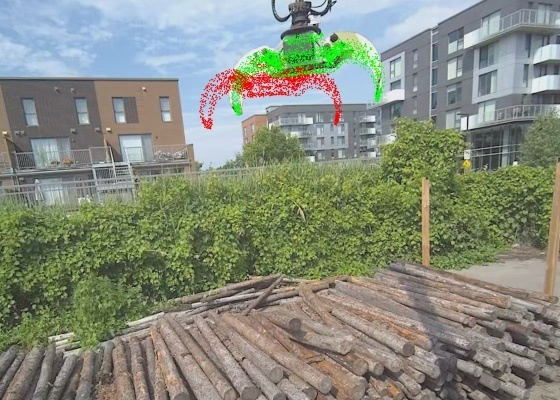
\includegraphics[width=\linewidth]{figures/calib/grapple_reproj_zed0.jpg}
\end{minipage}\hfill
\begin{minipage}{0.49\linewidth}
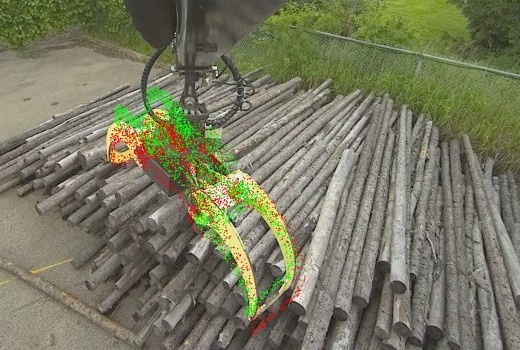
\includegraphics[width=\linewidth]{figures/calib/grapple_reproj_zed1.jpg}
\end{minipage}
\caption{Reprojection validation of the grapple-based calibration. The
grapple model, posed by forward kinematics and projected through the
floor-constrained calibrated mount (green) and through the nominal
uncalibrated mount (red), is overlaid on the mast camera (left) and stick
camera (right) images. In both views the calibrated model lands on the
observed grapple; the nominal mount is visibly displaced for the mast
camera, whose bracket pose is the one that changes whenever the mount is
adjusted.}
\label{fig:s2r_grapple_reproj}
\end{figure}

\begin{figure}[t]
\centering
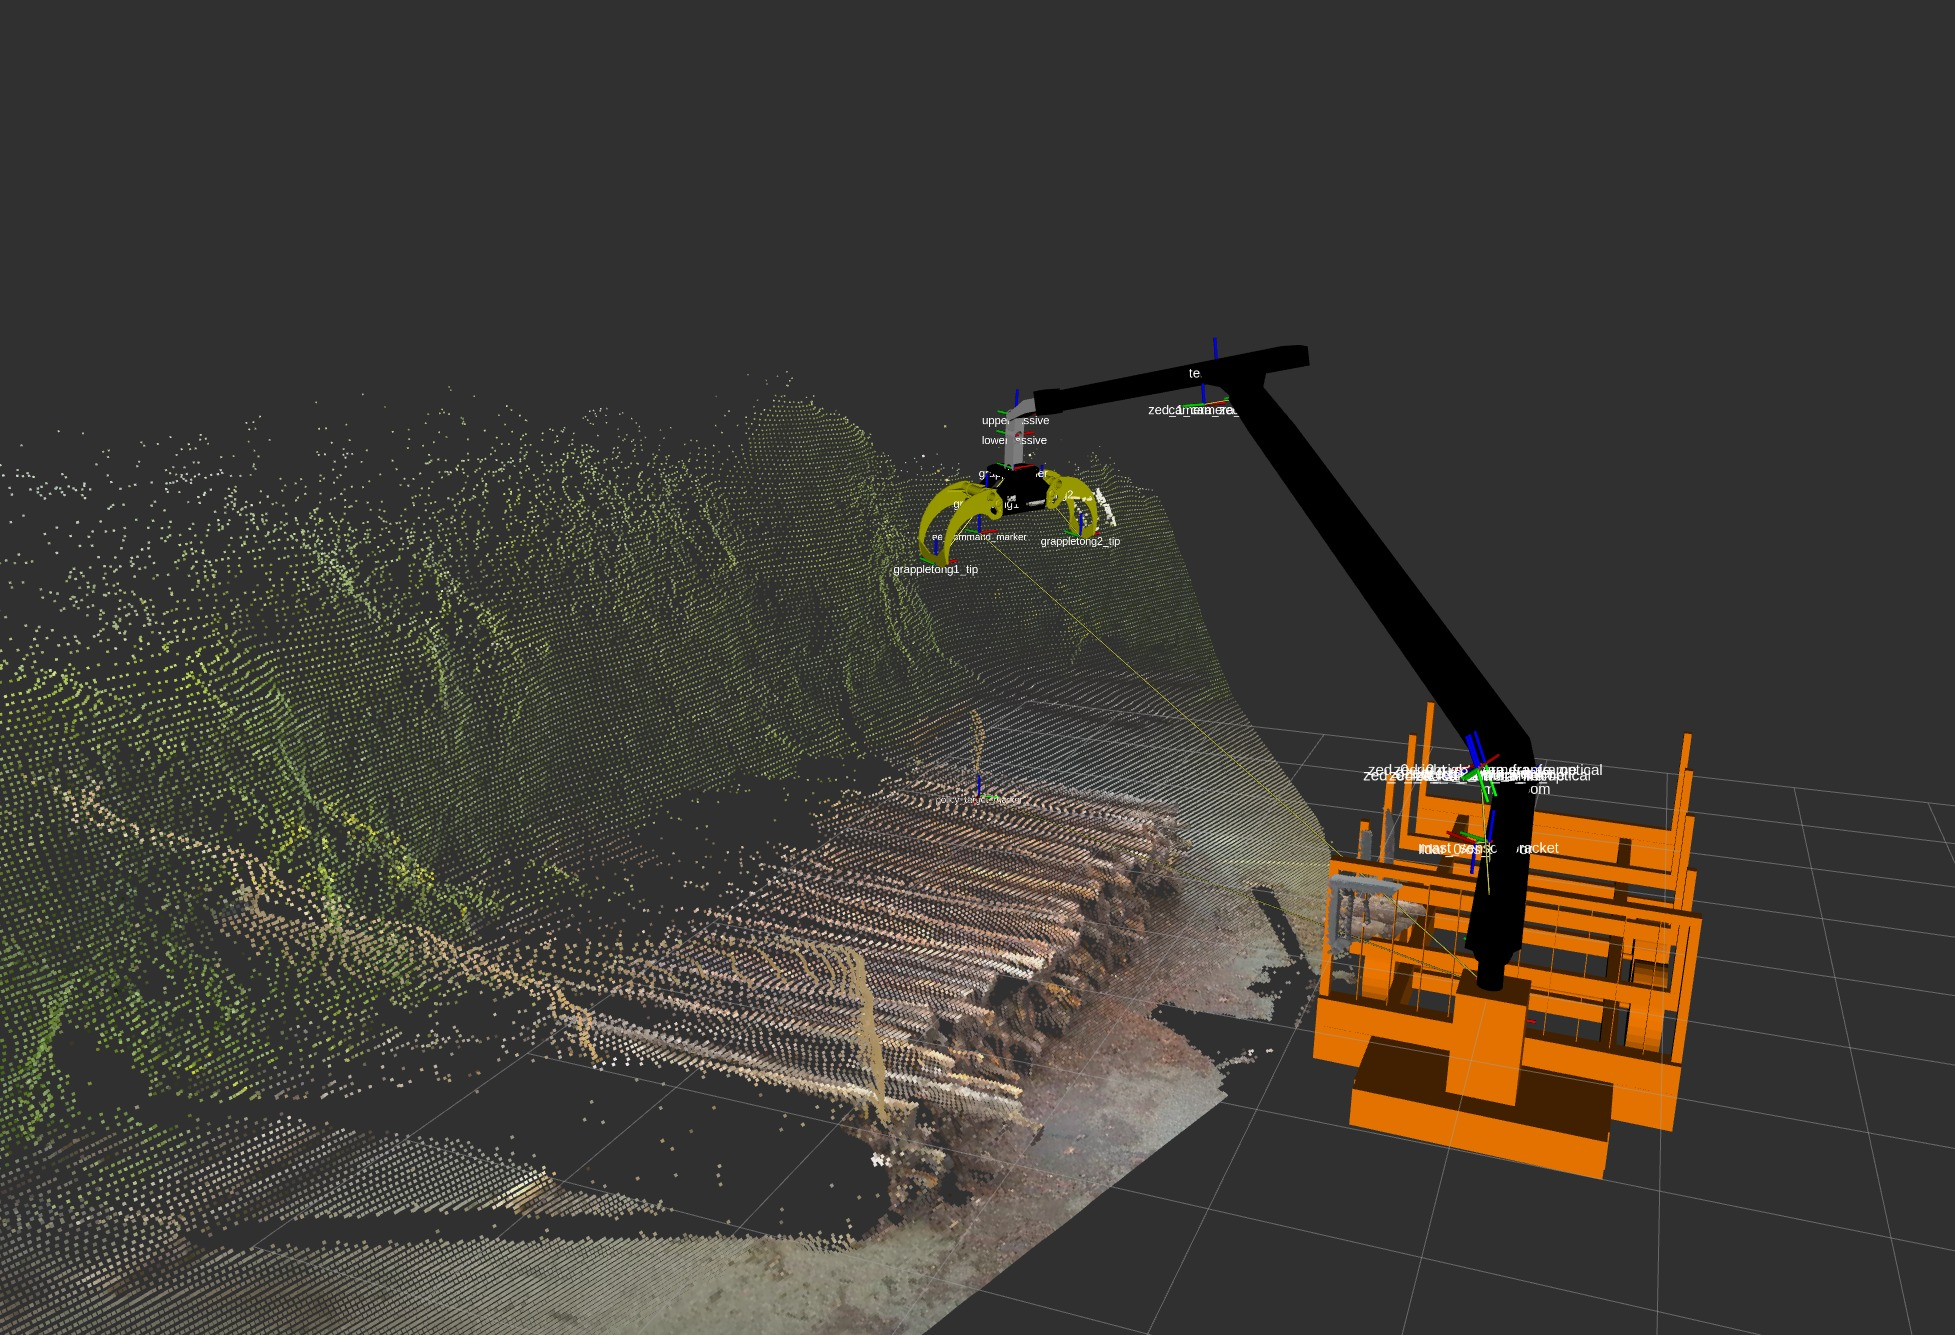
\includegraphics[width=0.92\linewidth]{figures/calib/replay_rviz.jpg}
\caption{Replay validation of the full calibration. Recorded camera and
joint-state data are replayed against the machine description carrying the
calibrated mounts, which is the sole transform authority: the crane model is
posed by the recorded joint states, and the registered camera cloud is
placed in the base frame through the calibrated extrinsics. The cloud lands
on the model consistently, with the observed pile, rack, and ground where
the model expects them.}
\label{fig:s2r_replay}
\end{figure}

\section{Rack Localization}
\label{sec:s2r_rack}

The action volume, the crop box, and the simulated rack must all sit where
the physical rack sits. The rack's 7.38~m length defeats single-camera
localization: no one viewpoint sees both ends with usable depth, so both
calibrated cameras are fused in the base frame. Printed fiducial
markers~\cite{garridojurado2014automatic} on the rack posts are detected in
full-resolution frames from each camera (Figure~\ref{fig:s2r_aruco}), each
detection lifted to the base frame through the camera's forward-kinematics
chain and calibrated mount. The mast camera contributes the near posts and
the stick camera the far post, and the marker pair spanning the rack's long
edge, a 7.5~m cross-camera baseline, fixes the rack yaw far more precisely
than any short edge. Because depth is the weak axis of fiducial pose
estimation at range (meter-scale errors at 7~m), marker detections only seed
the fit; the post columns visible in the registered point cloud refine the
corner positions, and the known rigid rack footprint ($2.16 \times 7.38$~m)
is fitted for pose only, anchored on the two reliable corner posts. The
recovered rack pose placed the rack bottom on the ground plane to within
24~mm of the simulator's, and reprojecting the fitted rack wireframe onto
the camera image shows the box edges following the physical posts
(Figure~\ref{fig:s2r_wireframe}). The procedure was re-run from a single
recorded sequence when the crane was later repositioned.

\begin{figure}[t]
\centering
\begin{minipage}{0.49\linewidth}
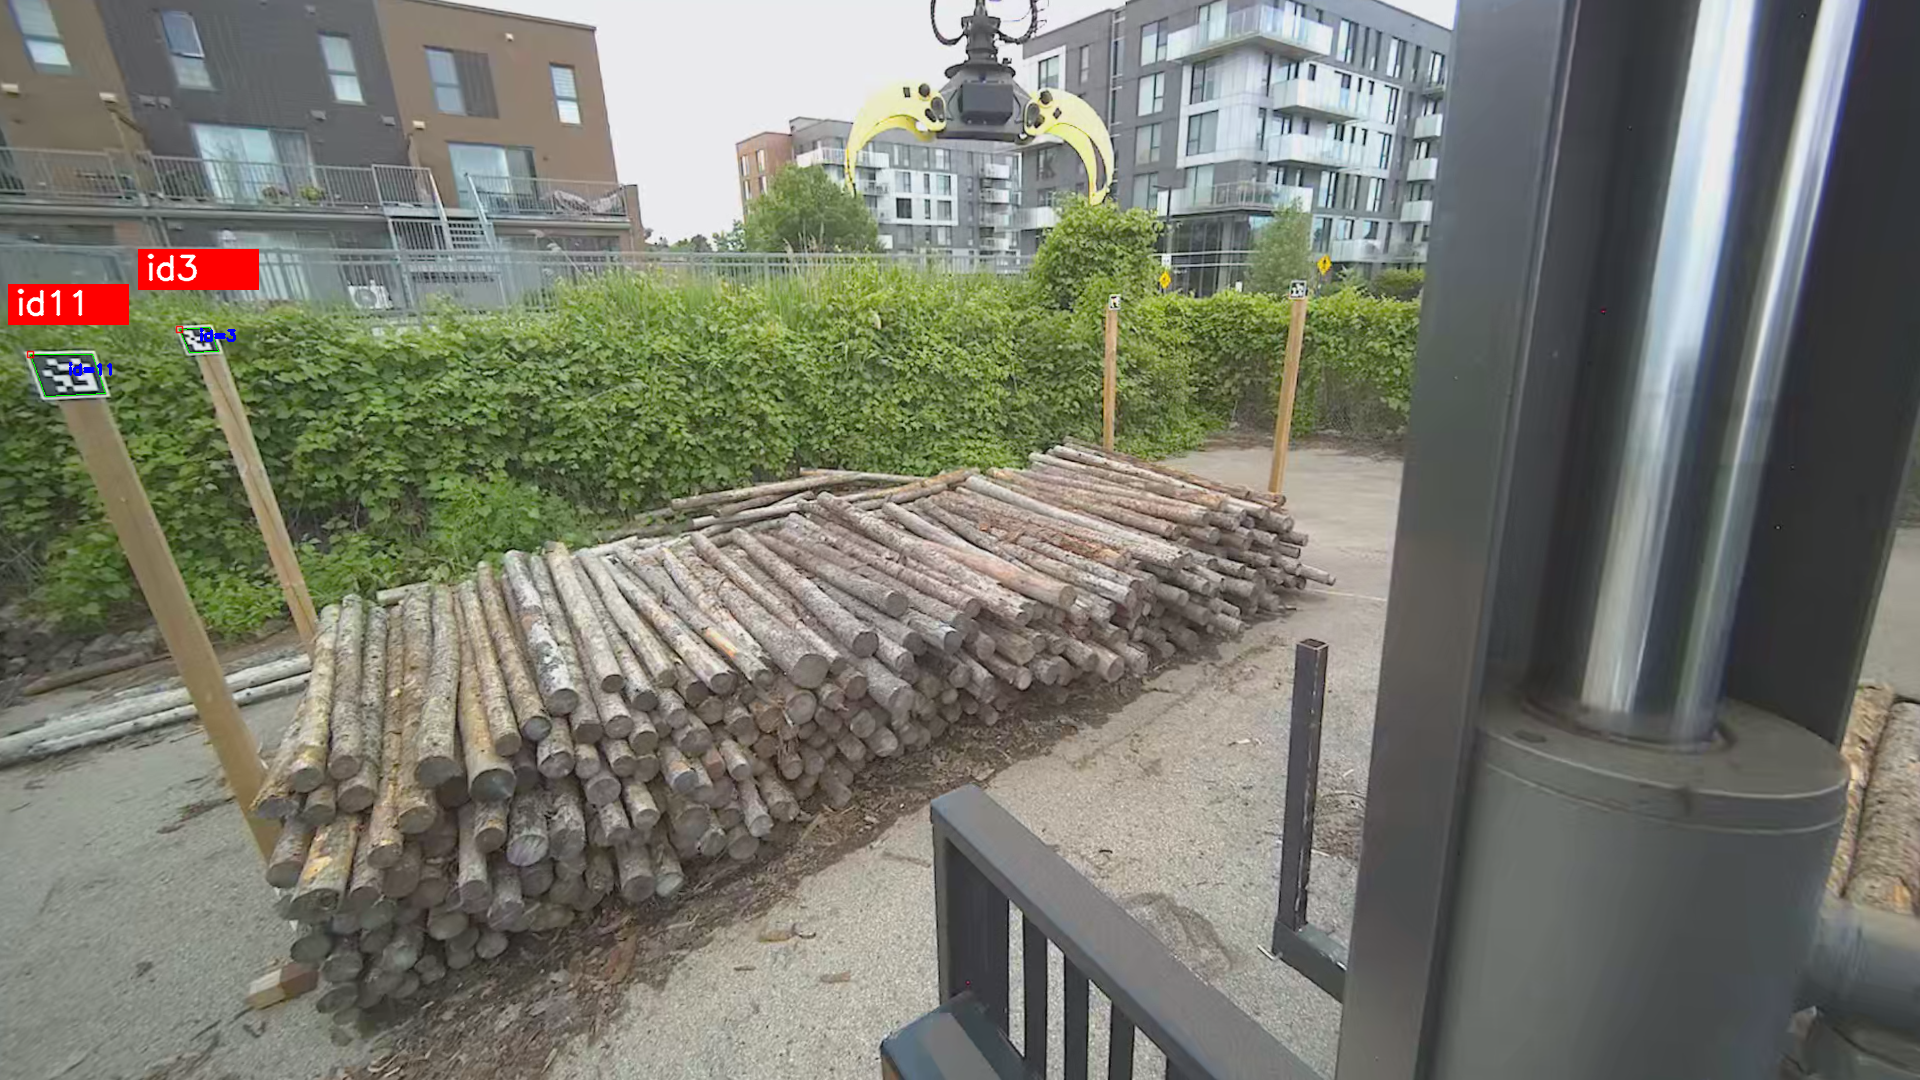
\includegraphics[width=\linewidth]{figures/calib/det_zed0.png}
\end{minipage}\hfill
\begin{minipage}{0.49\linewidth}
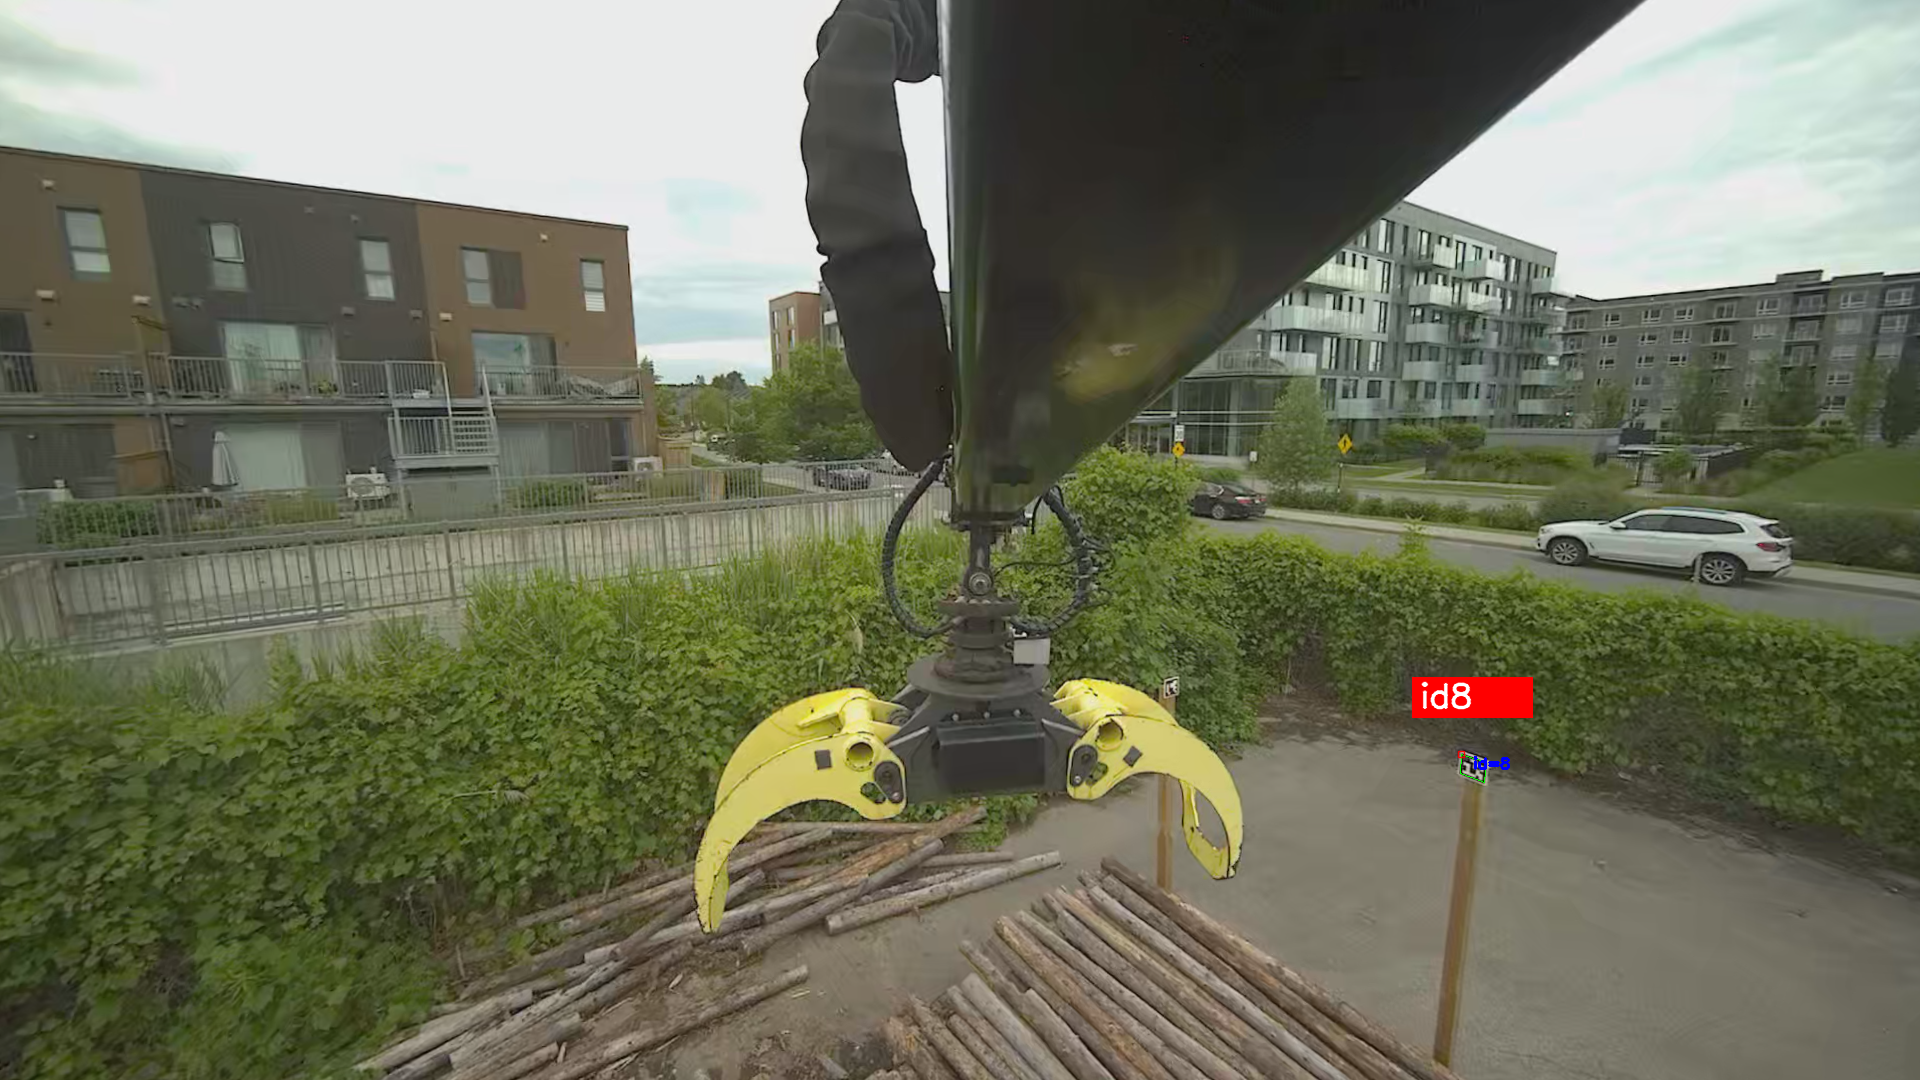
\includegraphics[width=\linewidth]{figures/calib/det_zed1.png}
\end{minipage}
\caption{Fiducial detections for rack localization. Left: the mast camera
sees the near rack posts. Right: the stick camera reaches the far post that
the mast camera cannot resolve, motivating the two-camera fusion.}
\label{fig:s2r_aruco}
\end{figure}

\begin{figure}[t]
\centering
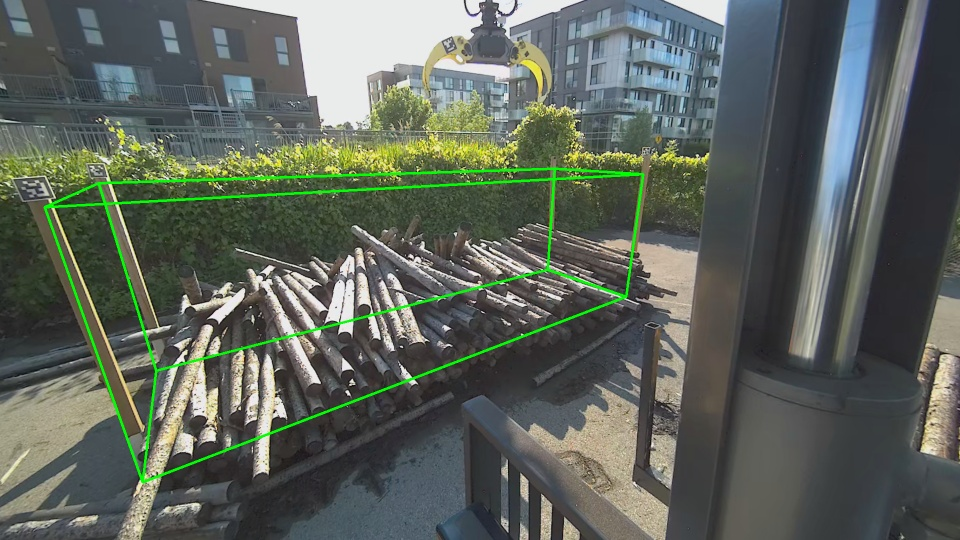
\includegraphics[width=0.8\linewidth]{figures/calib/rack_final_wire7.jpg}
\caption{Validation of the fused rack localization: the fitted rack box,
reprojected through the calibrated mast camera, follows the physical posts
and rails.}
\label{fig:s2r_wireframe}
\end{figure}

\section{Matching the Training Environment to Deployment}
\label{sec:s2r_gaze}

With mounts and rack calibrated, the simulation is updated so that the
training observation is generated the way the deployed observation will be.

\emph{Sensor and scene placement.} The calibrated camera mounts are baked
into the machine description used by both the deployed nodes and the
simulator, the simulated mast camera is attached to the mast link at the
calibrated transform, and the rack is placed at the calibrated base-frame
pose. The simulated camera's resolution and intrinsics are matched to the
calibrated ZED parameters.

\emph{The gaze phase.} On the real crane the mast camera's view depends on
the crane's configuration, and the arm can occlude the rack. The training
environment therefore adds a \texttt{GAZE} phase to the grasp cycle: before
each targeting decision the crane drives to a fixed joint-space gaze pose,
measured from recorded data of the physical crane parked in its viewing
configuration, in which the camera frames the rack and the arm is clear of
the view. The observation for each decision is captured at this pose, once
per cycle, exactly as at deployment. The environment step boundary is placed
at the settled gaze pose, so a policy step observes the gaze-pose cloud,
commands a grasp, and returns after the cycle completes and the crane is
back at gaze. This configuration, with the calibrated long rack and piles of
approximately 200 logs, is the training environment for all deployment-bound
policies in Chapters~\ref{ch:bc_policies} and \ref{ch:bcrl}.

\emph{Verification.} Figure~\ref{fig:s2r_gaze_rgb} compares the real and
simulated camera views at the gaze pose, and Figure~\ref{fig:s2r_overlay}
overlays simulated and real point clouds in the base frame. With calibrated
extrinsics the clouds land on the same rack volume, sharing the rack-region
extent in both horizontal axes. The residual differences are exactly the
sensor-realism gaps: real stereo depth carries holes and range-dependent
noise where simulated depth is complete and clean, and the real floor sits
about 13~cm below the simulated one. These observations motivate the
range-dependent noise augmentation of
Chapter~\ref{ch:bc_policies} and the observation crop, which
removes the floor from the policy input in both domains.

\begin{figure}[t]
\centering
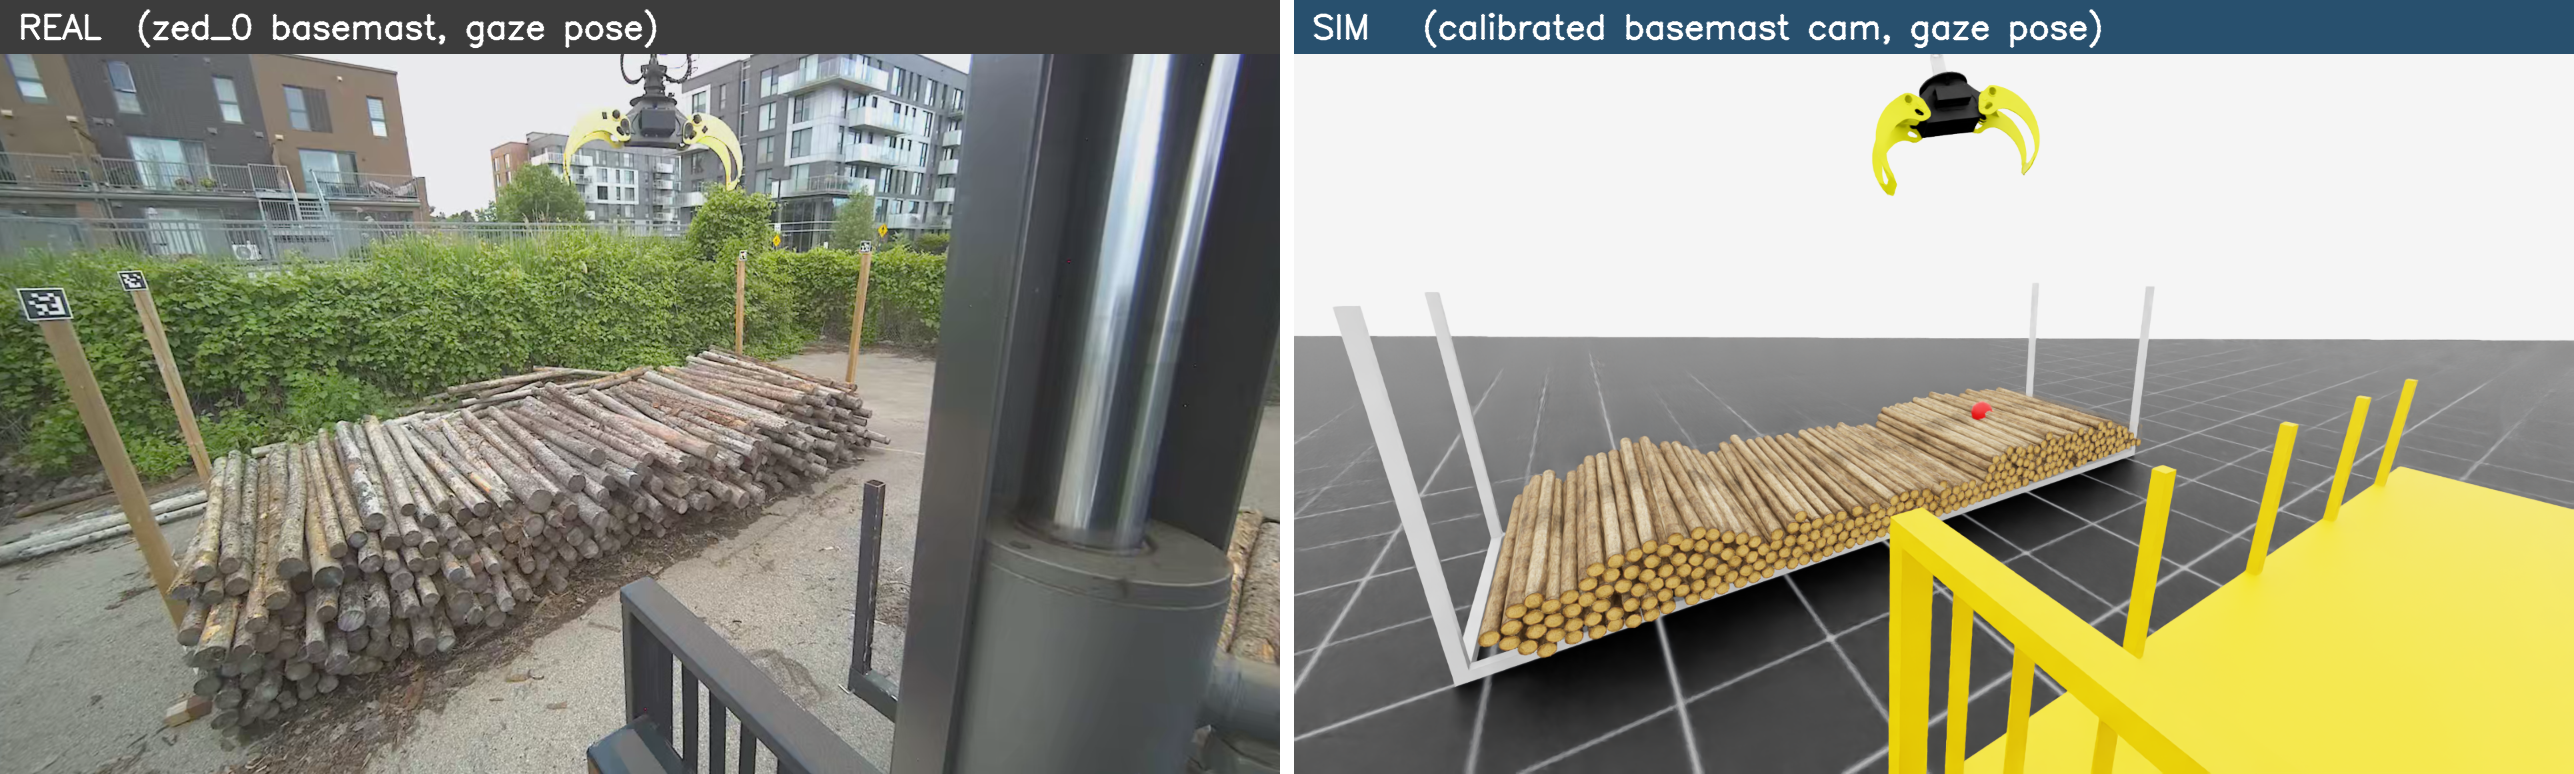
\includegraphics[width=\linewidth]{figures/calib/gaze_real_vs_sim.png}
\caption{Real (left) and simulated (right) mast-camera views at the gaze
pose after calibration. The simulated camera reproduces the deployed
viewpoint: grapple top-center, pile and rack in the lower half, matching
framing of the workspace.}
\label{fig:s2r_gaze_rgb}
\end{figure}

\begin{figure}[t]
\centering
\begin{minipage}{0.51\linewidth}
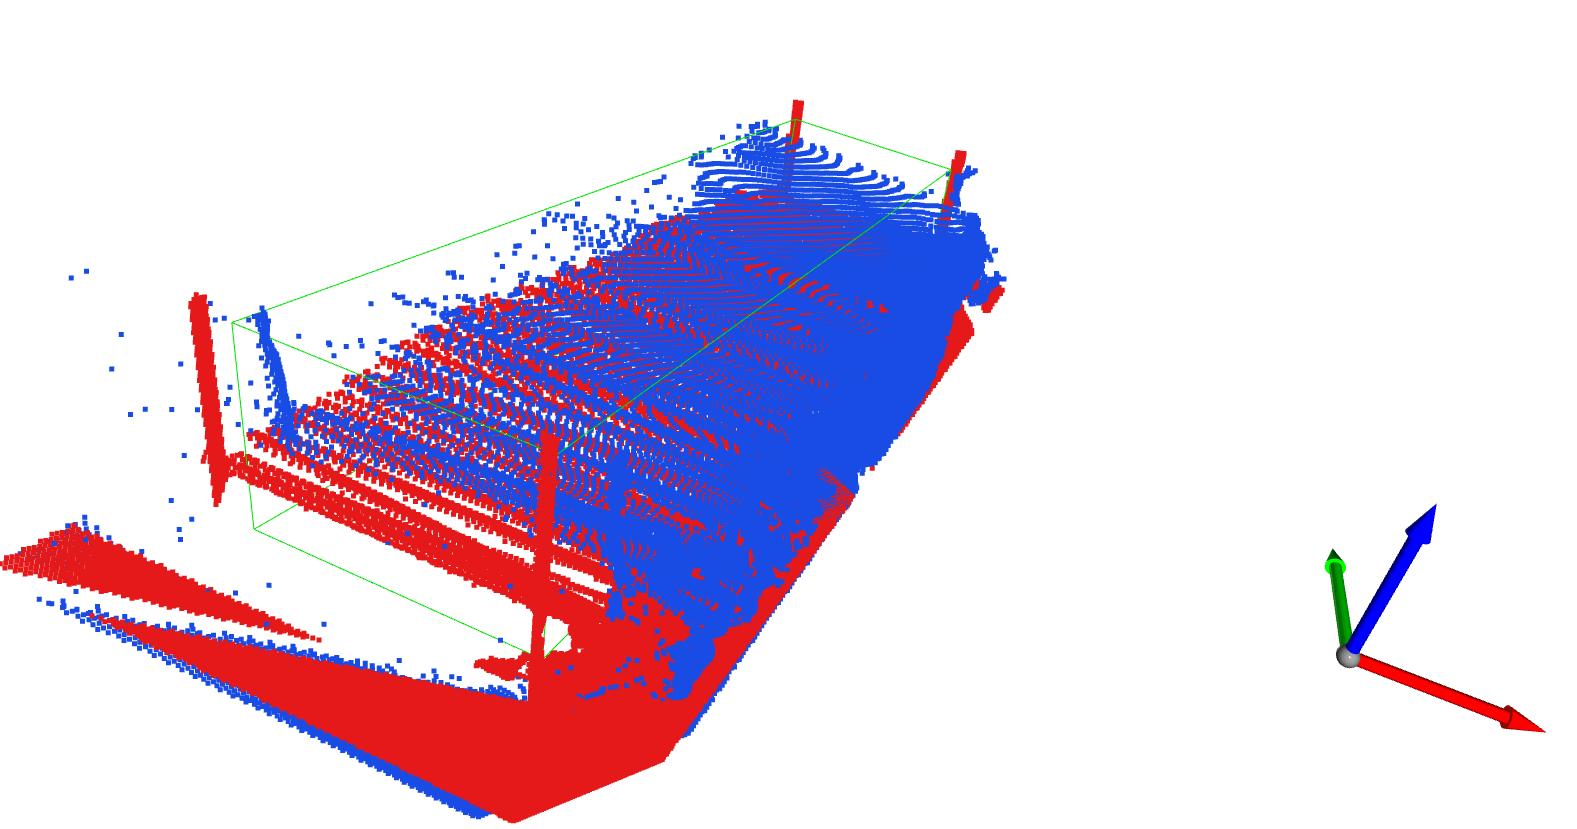
\includegraphics[width=\linewidth]{figures/calib/pcd_overlay_iso.png}
\end{minipage}\hfill
\begin{minipage}{0.47\linewidth}
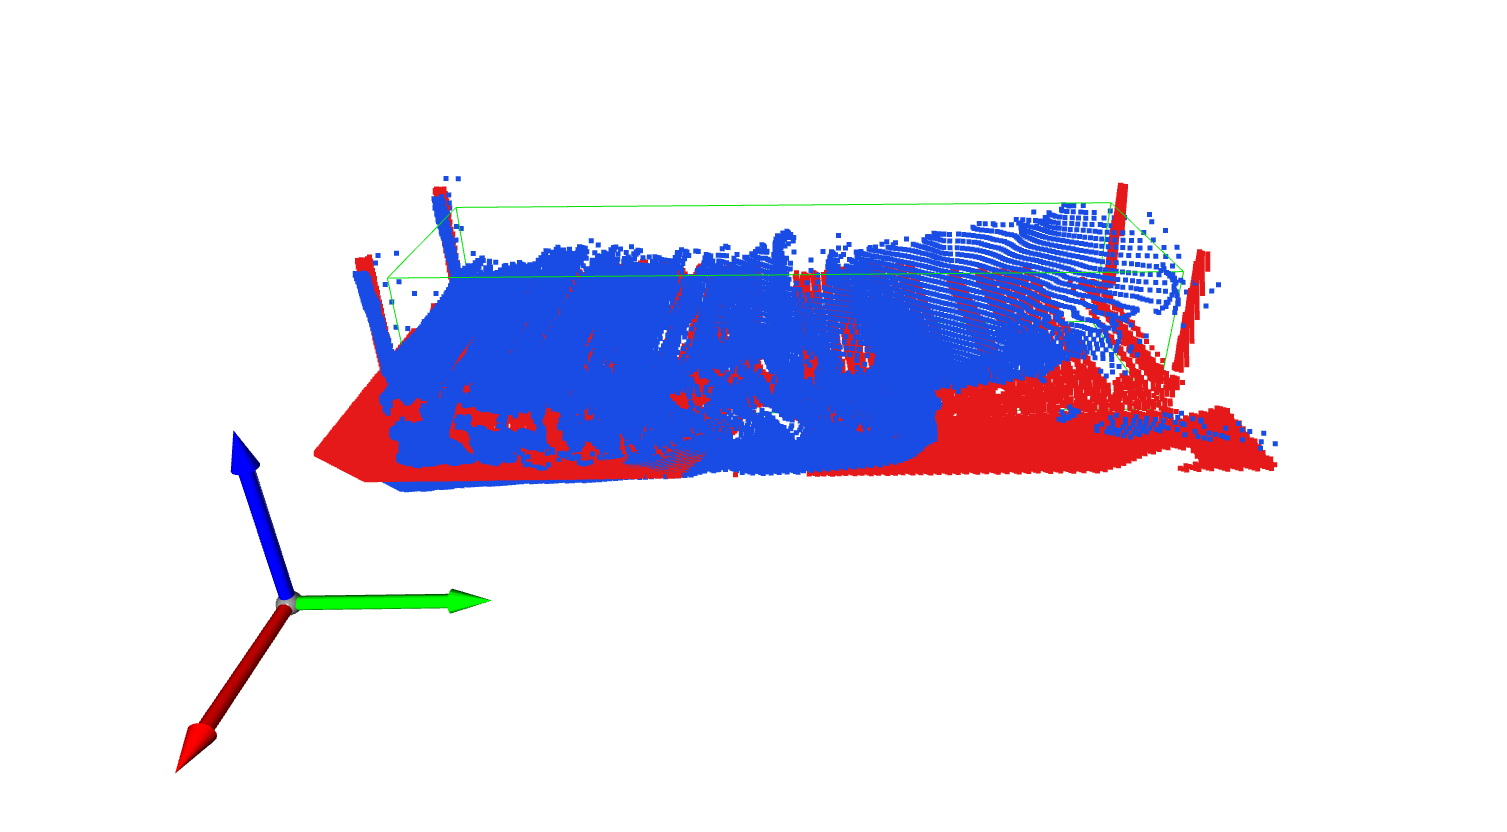
\includegraphics[width=\linewidth]{figures/calib/pcd_overlay.png}
\end{minipage}
\caption{Simulated (red) and real (blue) point clouds overlaid in the crane
base frame with the action volume in green; isometric (left) and side
(right) views. Calibration places both clouds on the same rack volume; the
remaining discrepancies are stereo holes and noise in the real cloud and a
floor-height offset of roughly 13~cm, both handled in the observation
pipeline.}
\label{fig:s2r_overlay}
\end{figure}

\section{Deposition}
\label{sec:s2r_deposit}

The learned decision ends at target selection; what happens to a grasped
bundle is sequenced by engineered logic in the policy node. After a
successful lift the crane carries the bundle to its home configuration and
deposits it into the trailer-bed area beside the rack, and the deposition
logic decides where along the trailer and from what height each bundle is
released.

The deposit area is divided into compartments by divider poles whose
positions were measured on the platform, giving four bins of roughly 1.28~m
width along the trailer axis. Bundles are laid across the active bin, with
the grapple yaw held perpendicular to the trailer length, and the bins are
filled in rotation from the far end toward the crane, one bundle per bin per
pass, so the load builds up in even layers; the bin nearest the crane is
excluded because the arm cannot load it cleanly. A bin counts as full once
its scanned fill height reaches a threshold, and when the last bin fills,
the run ends.

The release height adapts to the fill state
(Figure~\ref{fig:s2r_deposit}). Before each drop, with the crane settled at
the home pose, the mast-camera cloud is scanned over the active bin only,
inset from the divider poles so they are not mistaken for cargo, and the
release height is set a fixed clearance above the detected fill top. The
scan is gated for freshness the same way the gaze observation is: its sensor
timestamp must postdate the settling of the crane, so the held bundle and
the swinging grapple cannot inflate the measured fill height. A bin the
camera cannot yet see into falls back to a conservative blind release
height, and the first drop into an empty bin descends lower so the bundle
does not scatter. The per-bin fill state persists to disk, so an
interrupted run resumes its fill sequence instead of restarting it. All
field trials of Chapter~\ref{ch:bc_policies} run with this deposition
pipeline; a cycle succeeds only if it deposits at least one log, so
deposition is part of the measured system.

\begin{figure}[t]
\centering
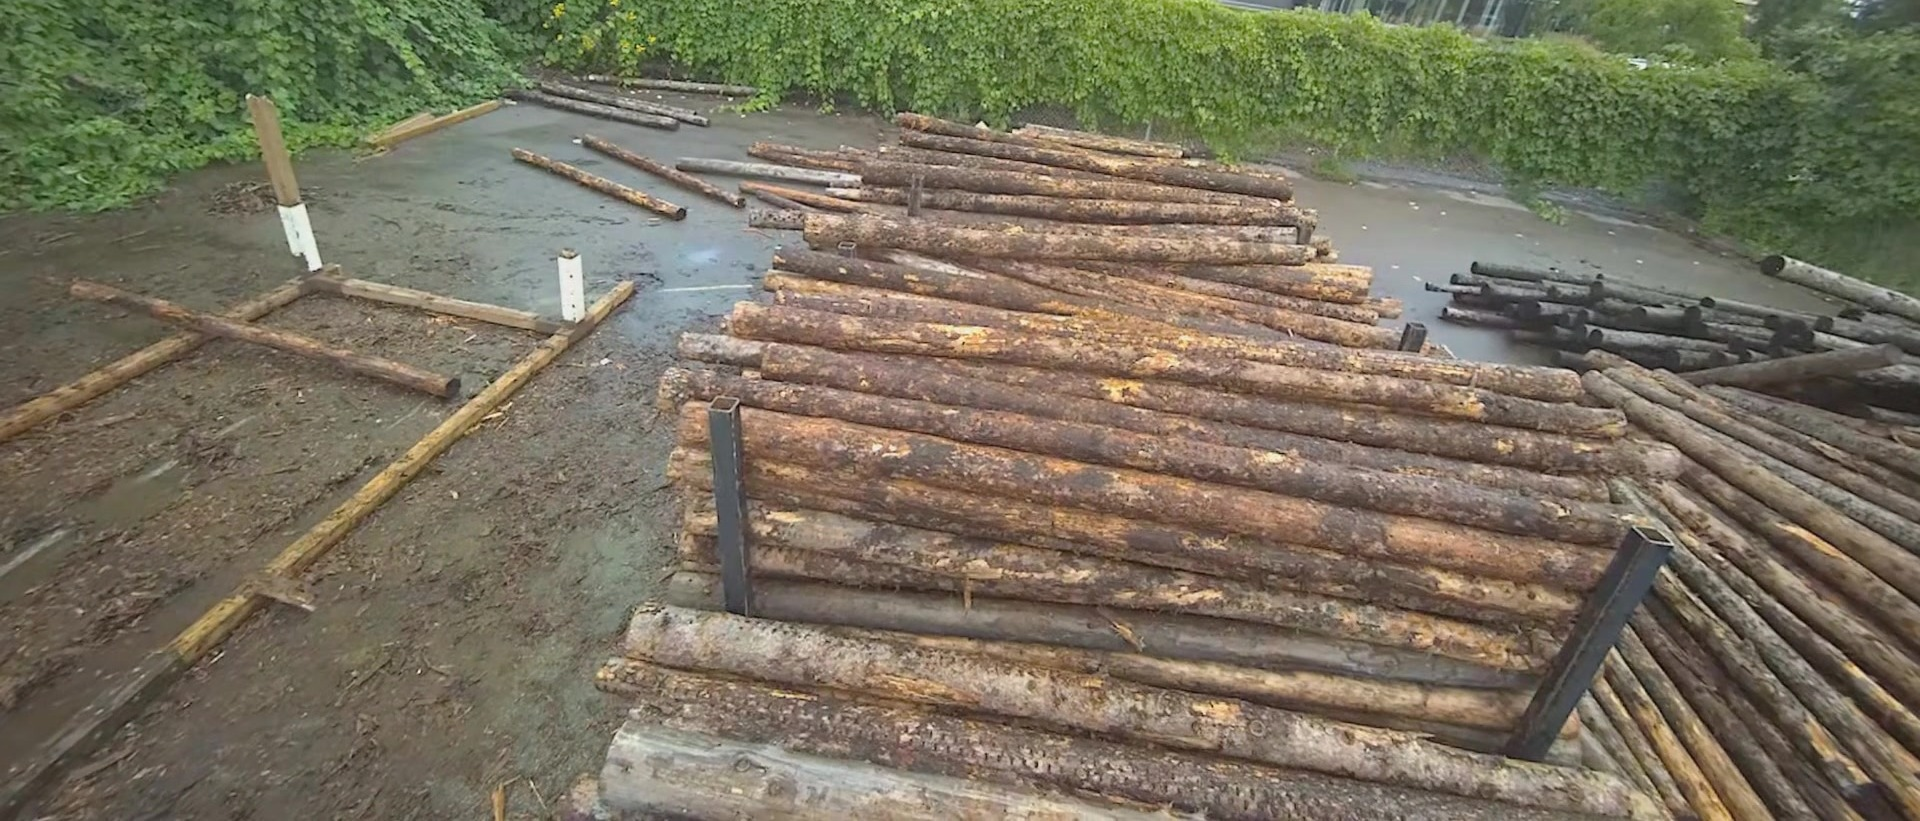
\includegraphics[width=0.9\linewidth]{figures/deposit_bins_photo.jpg}

\vspace{2mm}
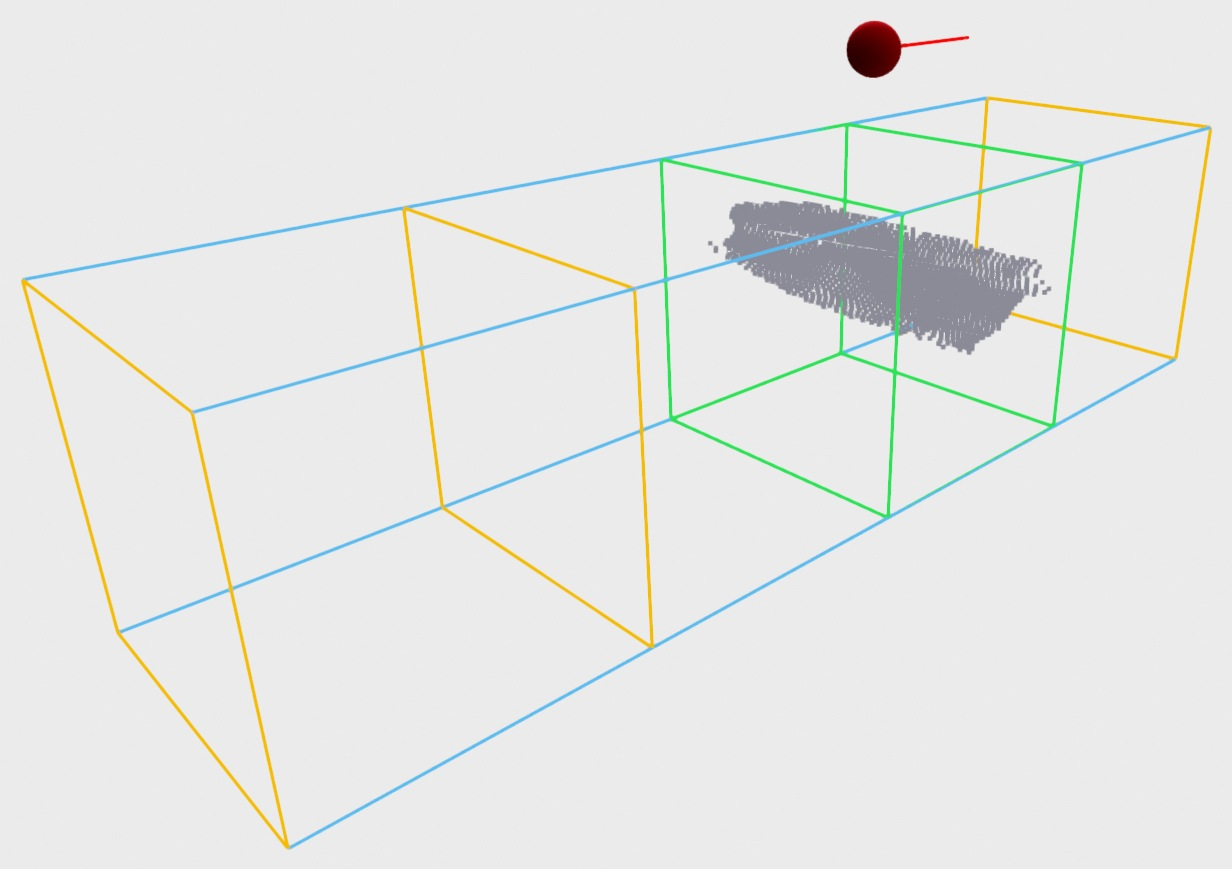
\includegraphics[width=0.88\linewidth]{figures/deposit_bin_iso.jpg}
\caption{Bin deposition during a field trial. Top: the mast-camera capture
this cycle's deposit scan was computed from, taken with the crane settled at
the home pose just before lowering to release; earlier bundles lie across
the pole-divided compartments beyond the rack, and the remaining pile is in
the foreground. Bottom: the deposit scan derived from that capture, in the
crane base frame. The deposit volume (blue) is split by the measured
divider planes (orange); only points inside the active compartment (green)
are retained (gray), and the release target (red sphere, with the commanded
grapple yaw as the red line) is placed a fixed clearance above their
detected top.}
\label{fig:s2r_deposit}
\end{figure}

\section{Deployment Pipeline Safeguards}
\label{sec:s2r_deploy}

Four further elements of the deployed pipeline matter for the field results
of Chapter~\ref{ch:bc_policies}.

\emph{Identical observation processing.} The deployed policy node runs
Algorithm~\ref{alg:obs_pipeline} unchanged: base-frame transform with the
calibrated extrinsics of Section~\ref{sec:s2r_camcalib}, crop to the
calibrated box, farthest point sampling to the trained budget, zero padding.
The decode that follows is Algorithm~\ref{alg:scoring_decode}, again
unchanged, with the action box supplied as a runtime parameter. Any deviation
between the two pipelines is a distribution shift the policy pays for
directly.

\emph{Actuation envelope.} Commanded grasp heights are clamped to the
platform bed level plus a safety margin at a single choke point, applied
identically to every target source (learned policies and the heuristic
baseline) and mirrored in the simulator's action decode. The commanded
height is the grasp center and the grapple tines sweep below it, hence the
margin; the clamp trades access to the bottom log layer for jam safety, a
platform constraint documented with the trials.

\emph{Frame recalibration.} The policies are trained in a fixed base-frame
coordinate system, and Chapter~\ref{ch:bc_policies} shows they are not
robust to translations of the scene within that frame. When the physical
rack was found to have shifted 0.45~m along the rack axis from its
calibrated position, the correction was a measured offset parameter that
translates the crop box onto the rack, returns the cropped cloud to training
coordinates for the network, and adds the offset back to the decoded
command. Scene geometry is thus treated as a calibrated quantity with a
defined recalibration procedure, not something the policy is expected to
absorb.

\emph{Run instrumentation.} Every deployed run writes a synchronized
record: a per-cycle dump of the policy input cloud and decoded target
(Figure~\ref{fig:s2r_policy_debug}), the deposit scan of each drop
(Figure~\ref{fig:s2r_deposit}), and decision and phase logs that index every
decision to the exact frame of the recorded camera stream. Any decision in a
trial can therefore be audited offline against exactly what the policy saw,
which is what makes the failure analysis and the offline policy replays of
Chapter~\ref{ch:bc_policies} possible.

\begin{figure}[t]
\centering
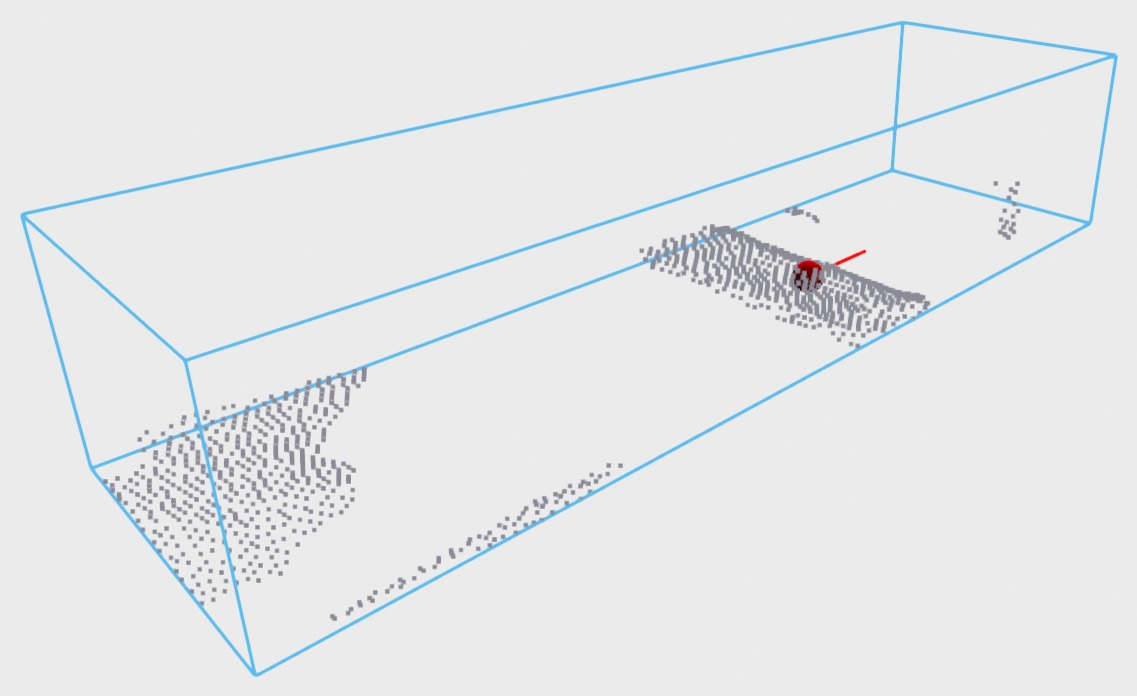
\includegraphics[width=0.85\linewidth]{figures/policy_debug_iso.jpg}
\caption{Per-cycle decision record from a field trial: the policy input
cloud (gray) inside the action volume (blue), with the decoded grasp target
(red sphere) and commanded yaw (red line), dumped at the moment of the
decision. This record is from the same cycle as the deposit scan of
Figure~\ref{fig:s2r_deposit}, late in the trial, when the policy targets
the last remaining row of logs.}
\label{fig:s2r_policy_debug}
\end{figure}

\section{Summary}

The transfer infrastructure rests on three measured results: the control
chain tracks commanded grasp targets to 1.5~cm over the rack workspace; the
grapple-based, floor-constrained calibration places both cameras' clouds in
the base frame with decimeter-scale registration residuals and ground-plane
tilt at the tenth-of-a-degree level; and the fused rack localization agrees
with the simulator's scene to centimeters, validated by wireframe
reprojection. On top of these, the training environment reproduces the
deployed viewpoint through the calibrated camera mount, the measured gaze
pose, and the calibrated rack placement, and the deployed pipeline
reproduces the training observation processing exactly. What remains between
simulation and the crane is the sensor-realism gap (stereo noise and holes)
and the behavioral consequences of pile geometry, which are the subject of
the next chapter.
